\documentclass[10pt,twocolumn,a4paper]{article}
\usepackage[pagenumbers]{cvpr}

\usepackage{graphicx}
\usepackage{amsmath}
\usepackage{amssymb}
\usepackage{booktabs}
\usepackage[pagebackref,breaklinks,colorlinks]{hyperref}
\usepackage[capitalize]{cleveref}

\crefname{section}{Sec.}{Secs.}
\Crefname{section}{Section}{Sections}
\Crefname{table}{Table}{Tables}
\crefname{table}{Tab.}{Tabs.}
\def\cvprPaperID{*****}
\def\confName{CVPR}
\def\confYear{2023}
\newcommand{\note}[1]{{\it\color{red} #1}}

%%%%%%%%%%%%%%%%%%%%%%%%%%%%%%%%%%%%%%%%%%%%%%%%%%%%%%%%%%%%%%%%%%%%

\begin{document}

\title{Paper Reproduce: Visualize the Crypto Data of BTC and Eth}
\author{Jiaxi Xu\\jx2548\\{\tt\small jx2548@nyu.edu}}
\maketitle



%%%%%%%%%%%%%%%%%%%%%%%%%%%%%%%%%%%%%%%%%%%%%%%%%%%%%%%%%%%%%%%%%%%%
\begin{abstract}

The rapid growth and pervasive adoption of crypto currencies, particularly Bitcoin (BTC) and Ethereum (ETH), have transformed the financial landscape and attracted the attention of investors, traders, and financial institutions. As crypto currencies continue to mature and acquire prominence in the global economy, the demand for accessible and user-friendly visualization tools increases. This project will utilize data visualization of the history of crypto currencies to enable novice and experienced users to analyze market trends and make informed decisions more intuitively.

\end{abstract}
%%%%%%%%%%%%%%%%%%%%%%%%%%%%%%%%%%%%%%%%%%%%%%%%%%%%%%%%%%%%%%%%%%%%

\section{Introduction}
\label{sec:introduction}


The project intends to meet this need by analyzing historical data on two prominent crypto currencies, Bitcoin and Ethereum, and comparing their recent transaction prices, volumes, and general trends\cite{nils_2022}. Utilizing cutting-edge data visualization technologies, the project will provide valuable insights into the performance of these crypto currencies and enable users to recognize patterns and trends that can inform their investment strategies.

The visualization will include a line chart of virtual currency prices, representing the historical price movements of Bitcoin and Ethereum in a plain and concise manner\cite{orac_2021}. Users will be able to evaluate the relative performance of these crypto currencies and identify periods of growth, decline, and stability using the chart. In addition, a stack area depiction of transaction percentage will be created to provide an all-encompassing view of Bitcoin and Ethereum trading volume over time. This visualization will enable users to comprehend the market dynamics and trading activity surrounding these crypto currencies, as well as identify periods of increased market liquidity and interest.

By providing these user-friendly visual tools, the project hopes to contribute to the growing body of knowledge surrounding crypto currencies and aid investors, traders, and other stakeholders in the crypto currencies space in making informed decisions\cite{sun}. The project's ultimate goal is to improve users' access to and comprehension of crypto currencies market trends, enabling them to make more informed decisions in the swiftly evolving world of digital assets.

%%%%%%%%%%%%%%%%%%%%%%%%%%%%%%%%%%%%%%%%%%%%%%%%%%%%%%%%%%%%%%%%%%%%
\section{Related Work}
In recent years, research on crypto currencies and their market trends has expanded swiftly, and numerous studies have examined various aspects of the crypto currency market. The work of Yermack\cite{Yermack2013}, which investigated the potential of Bitcoin as a medium of exchange and store of value and analysed the regulatory challenges and opportunities it presents, is one of the most influential studies in this field. 

In addition, Bohme et al. \cite{Bohme2015} investigated the security and privacy aspects of Bitcoin transactions, as well as potential assaults and countermeasures in the Bitcoin network. Similarly, Zohar's \cite{Zohar2015BitcoinUT} work addressed Bitcoin's scalability issues and proposed a new framework for enhancing the transaction throughput of the Bitcoin network.

Moreover, numerous studies have investigated the relationship between the crypto currency market and the traditional financial market. For example, Kristoufek \cite{Kristoufek2014} analysed the correlation between Bitcoin and traditional assets like gold, energy, and stocks. Corbet et al. \cite{Corbet2018} also investigated the dynamic correlations between Bitcoin and other financial assets, such as commodities, currencies, and stock indices.

In conclusion, there is a vast corpus of literature on crypto currencies and their market trends, covering a range of topics including security, privacy, scalability, regulation, co-movements with traditional assets, mining, and consensus mechanisms. This paper seeks to contribute to this expanding body of knowledge by providing an insightful data visualisation of the historical trends of Bitcoin and Ethereum, two prominent crypto currencies.


%%%%%%%%%%%%%%%%%%%%%%%%%%%%%%%%%%%%%%%%%%%%%%%%%%%%%%%%%%%%%%%%%%%%
\section{Demonstration}
The user interface of the project will allow users to interact with data visualisation and obtain valuable insights into bitcoin and Ethereum's historical trends. The user will see a concise description of the project and its objectives when the screen loads.

Depending on the user's preference, the interface's home page displays multiple visualisations layered side by side or vertically. Users will be able to choose the time period they wish to analyse by selecting various parameters and packets in function, including "1 day", "12 hours", and "4 hours." This will enable users to examine the evolution of the performance of the two cryptocurrencies over specific time periods.

The following visualizations will be included in the user interface:

1. Line Chart Displaying Historical Prices: This visualization will display the historical price movements of Bitcoin and Ethereum using a line chart. The x-axis will represent time, while the y-axis will represent crypto currencies prices. The chart will exhibit two lines, one for each crypto currency, each with a distinct color and label. Users will be able to hover over the chart to view specific price points and identify key moments of growth, decline, and stability for each crypto currency.
\begin{figure}[!h]
  \centering
  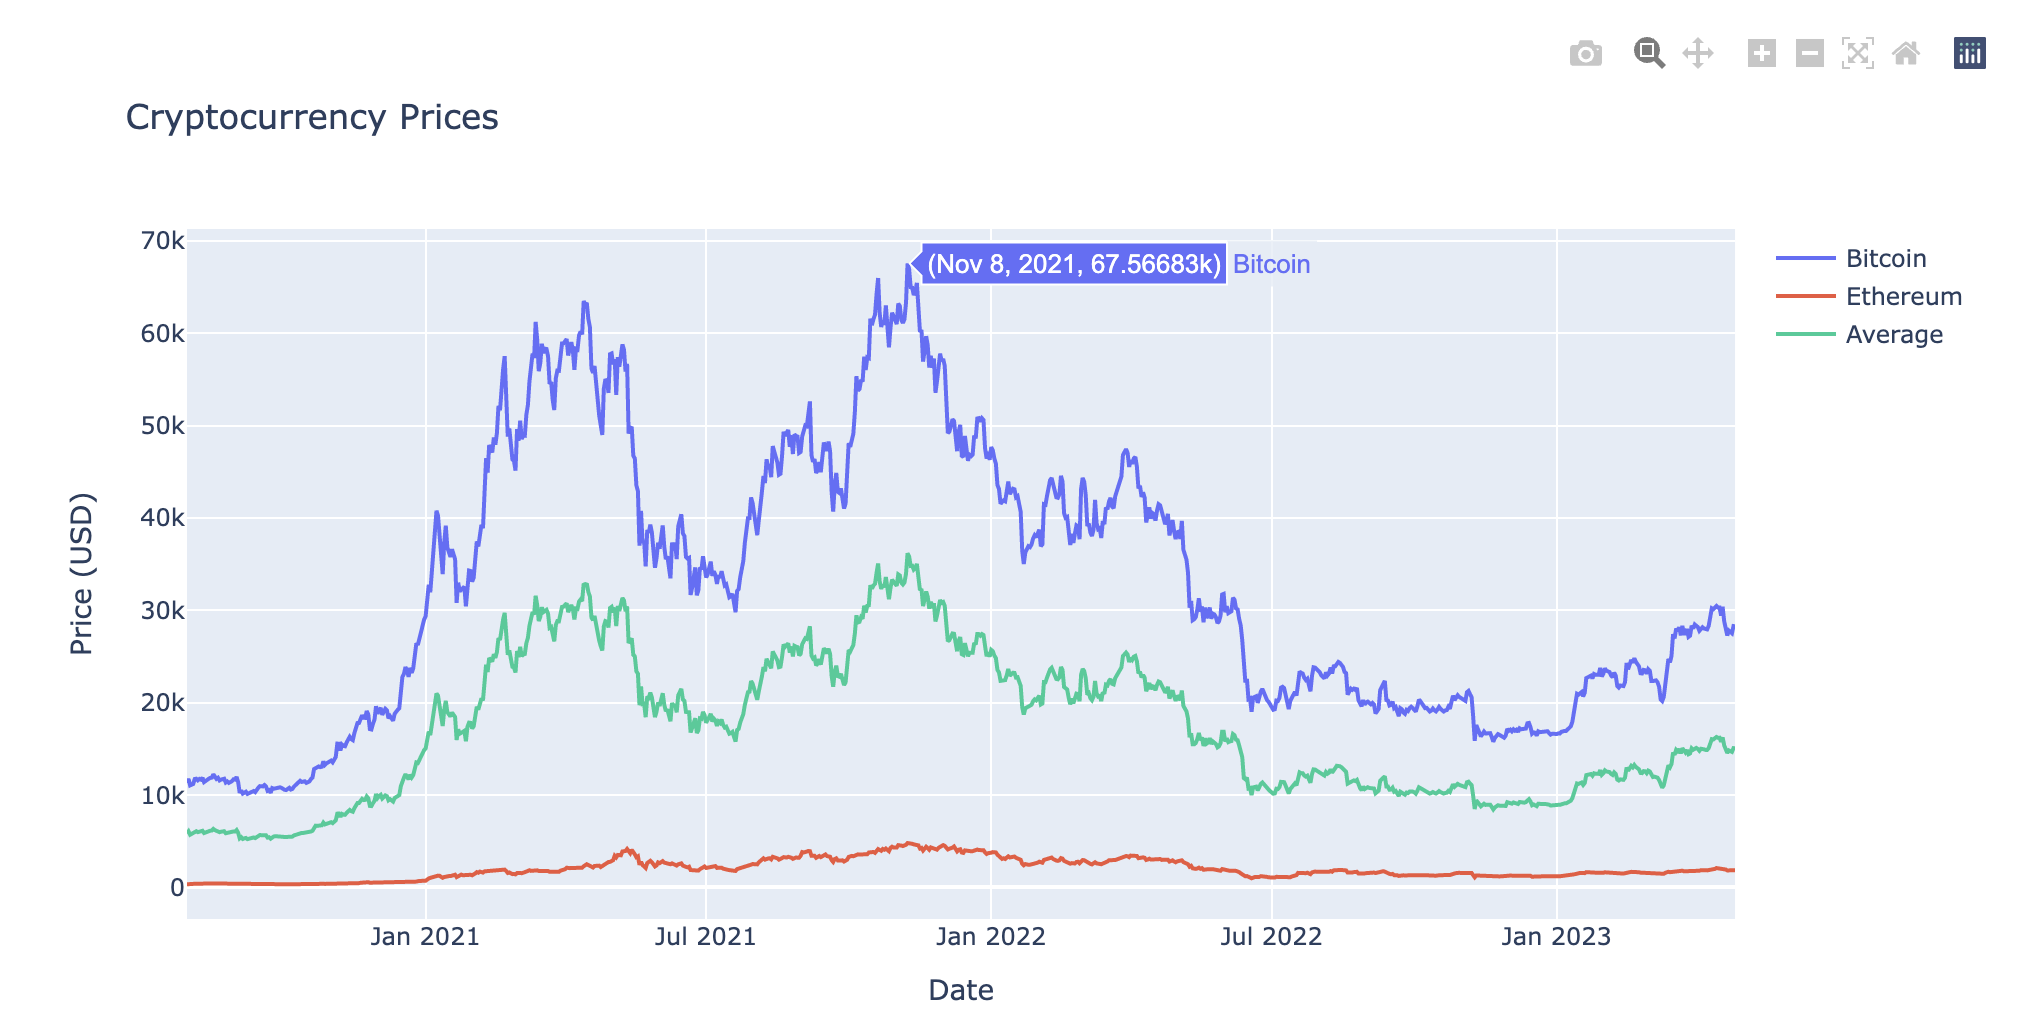
\includegraphics[width=1\linewidth]{Cryptocurrency.png}
  \caption{Crypto Prices and Average.}
  \label{fig:example}
\end{figure}

2. Stacked Area Chart of Volume Traded: This visualization will depict the trading volume of Bitcoin and Ethereum over time using a stacked area chart. Time will be represented by the x-axis, while trading volume will be represented by the y-axis. The chart will depict two discrete areas, one for each crypto currency, each with its own color and label. Users will be able to hover over the chart to view specific trading volume points and identify periods of increased market liquidity and interest.
\begin{figure}[!h]
  \centering
  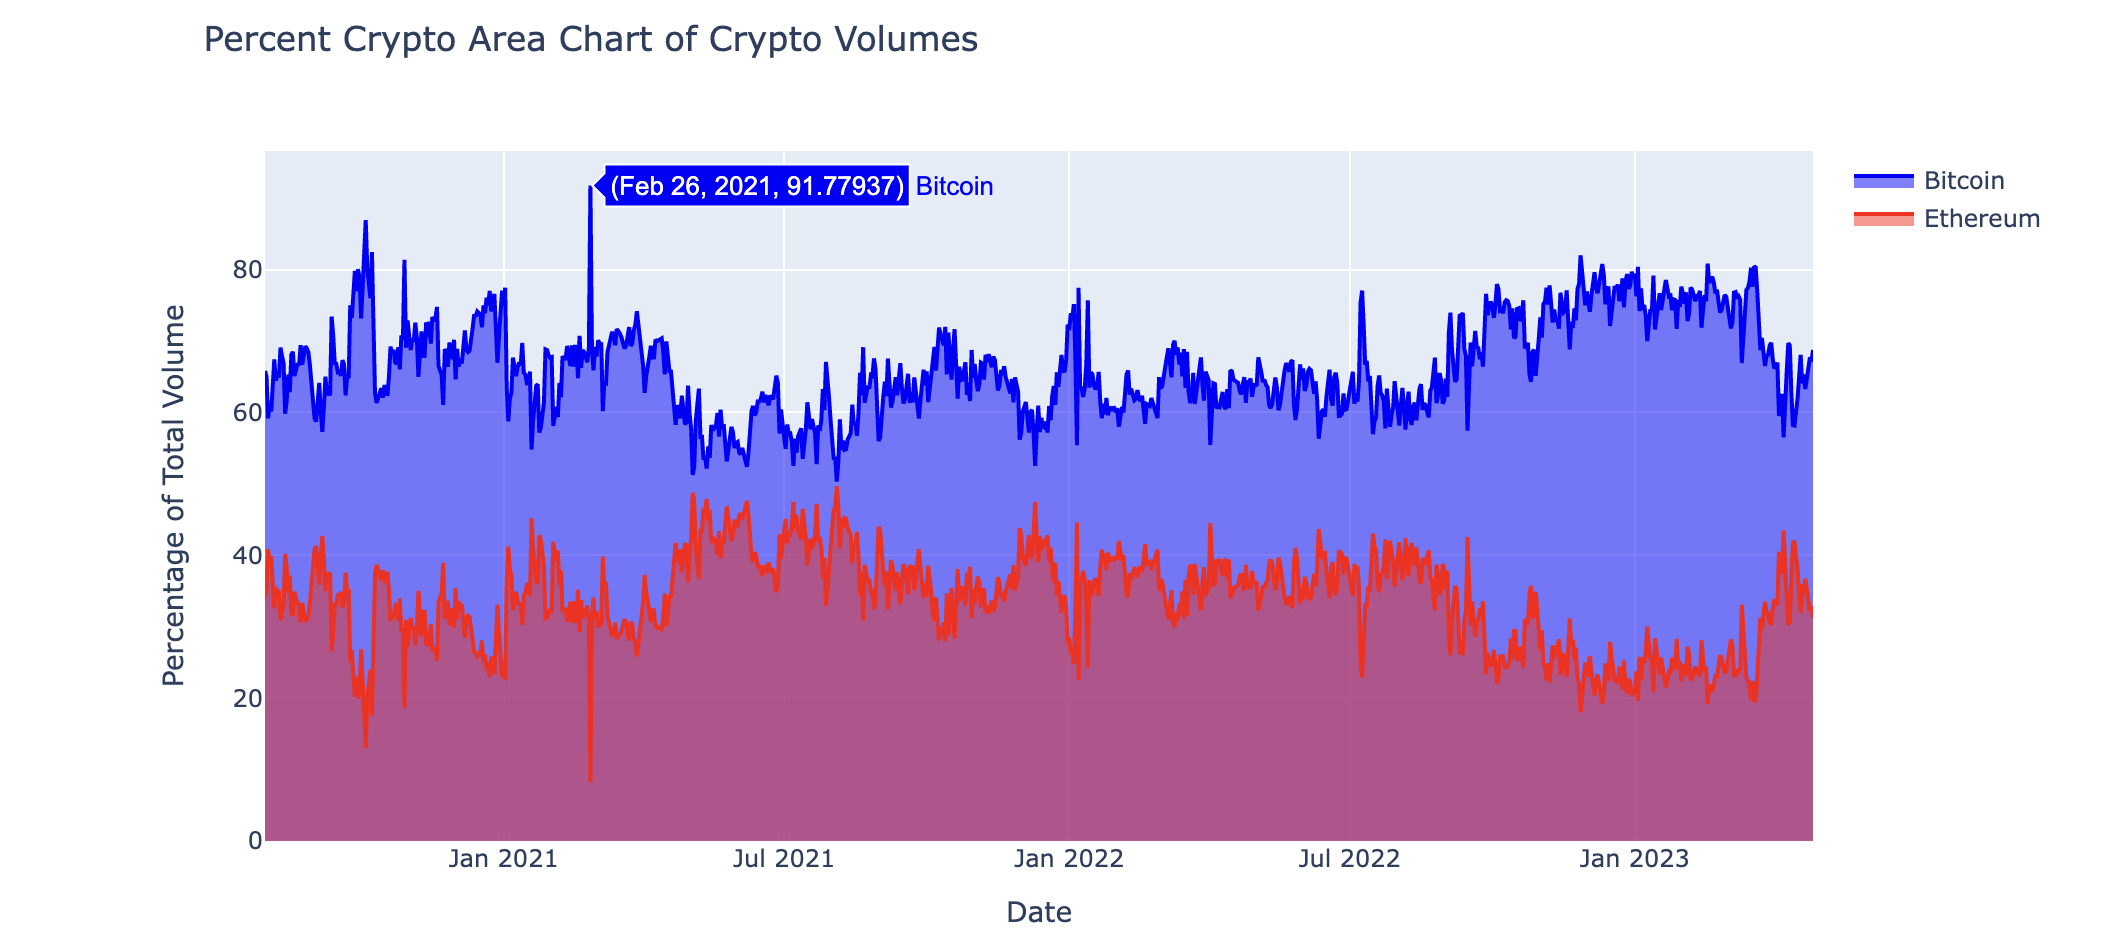
\includegraphics[width=1\linewidth]{Stacked_Area.png}
  \caption{Stacked Area Chart of Volume Traded.}
  \label{fig:example}
\end{figure}


3. Moving Average (MA) Chart: This visualization will display the MA of Bitcoin and Ethereum using a line chart. Users will be able to select the MA period (such as 10-day or 50-day MA) and view the MA line along with the historical price movements of the crypto currencies.
\begin{figure}[!h]
  \centering
  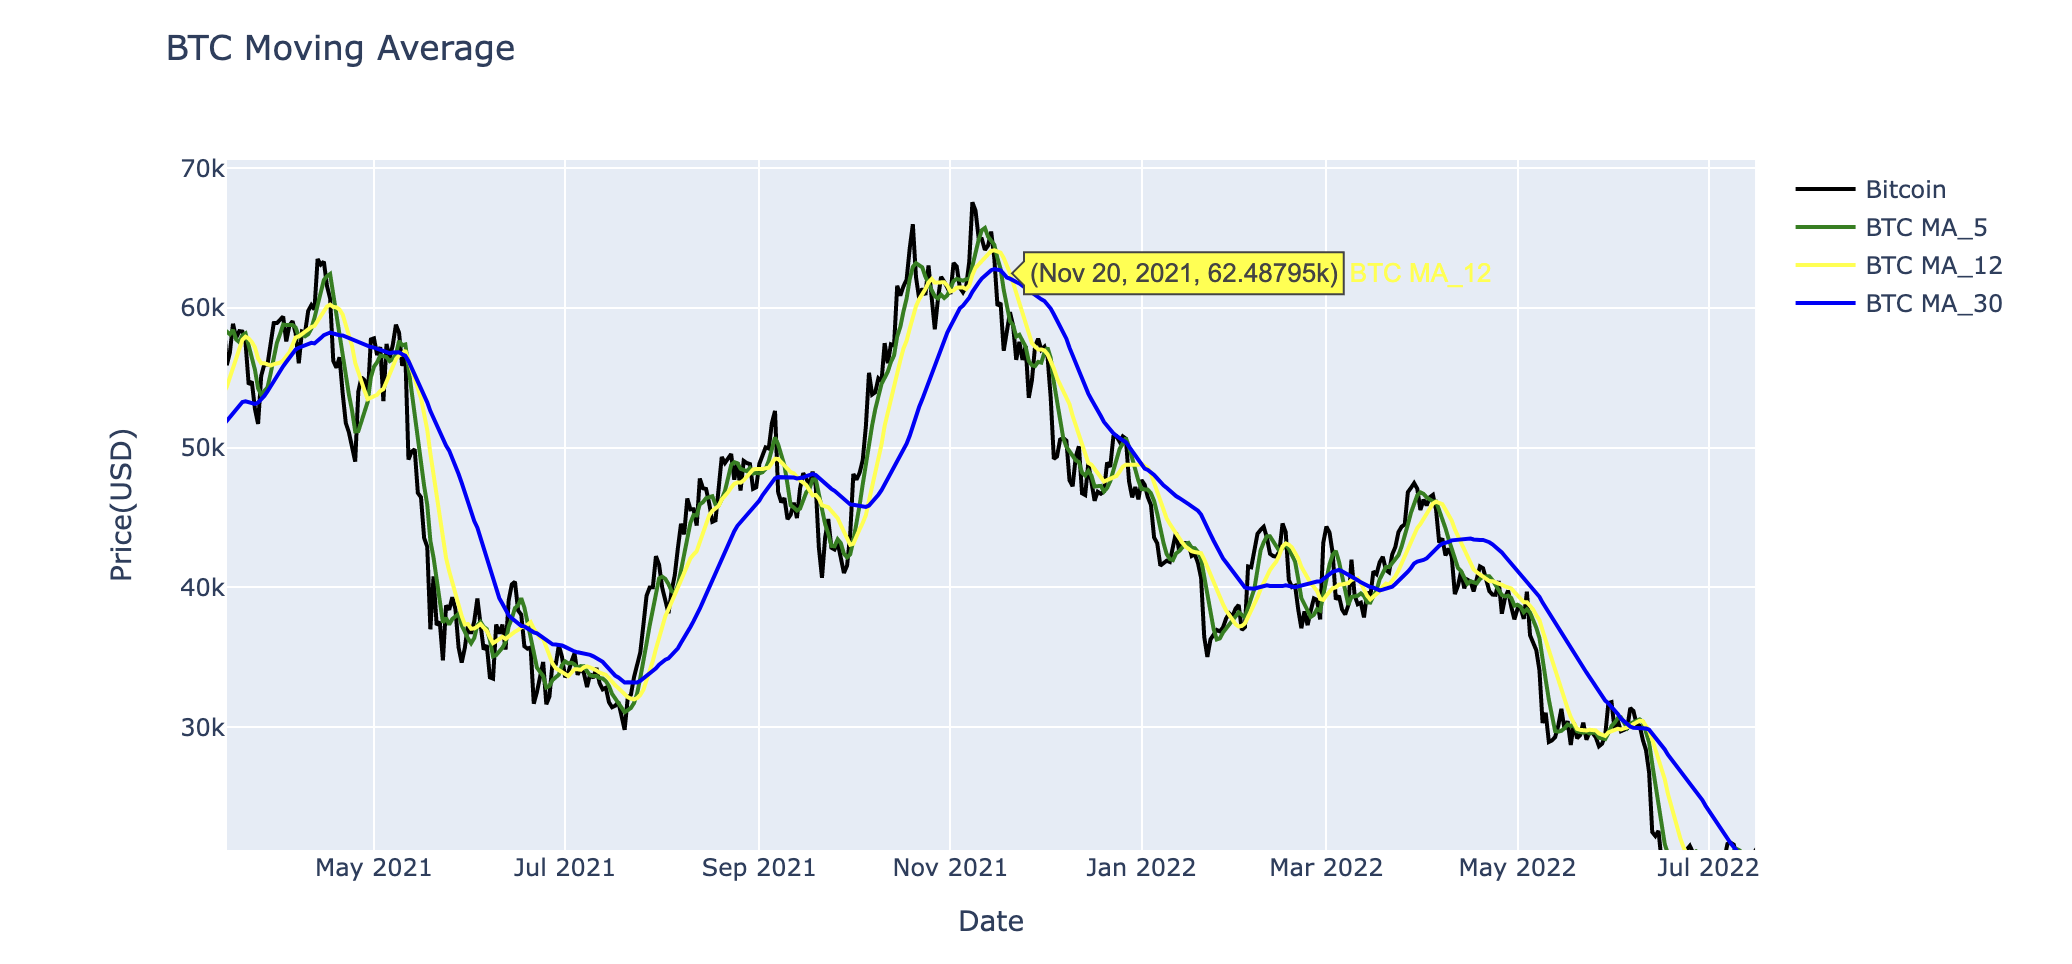
\includegraphics[width=1\linewidth]{MA.png}
  \caption{Moving Average.}
  \label{fig:example}
\end{figure}

4. Moving Average Convergence Divergence (MACD) Chart: This visualization will display the MACD of Bitcoin and Ethereum using a bar chart. Users will be able to select the MACD parameters (such as 12, 26, 9) and view the MACD bars along with the signal line and the historical price movements of the crypto currencies.
\begin{figure}[!h]
  \centering
  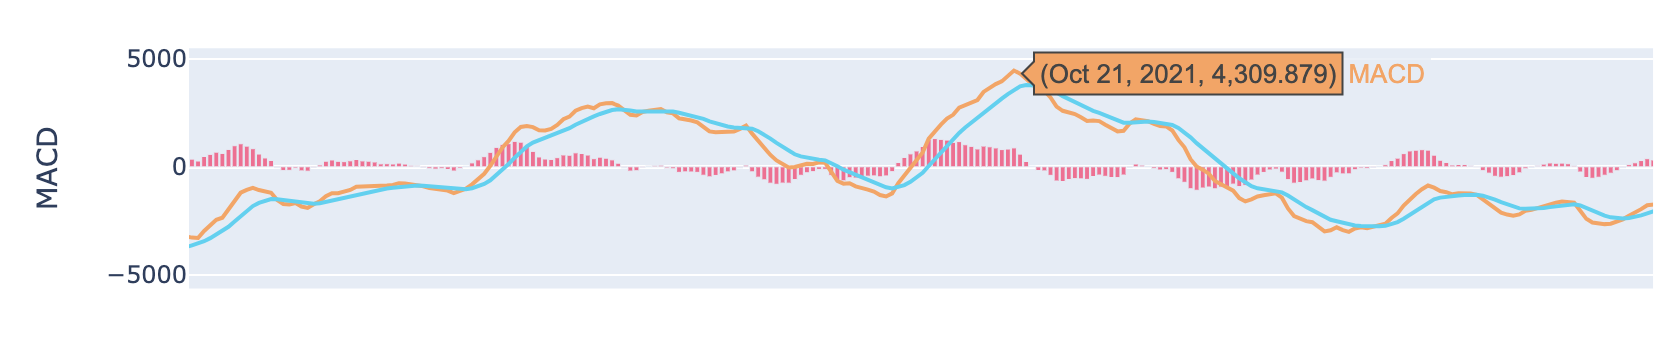
\includegraphics[width=1\linewidth]{MACD.png}
  \caption{Moving Average Convergence Divergence.}
  \label{fig:example}
\end{figure}

5. Candlestick Chart: This visualization will display the trading activity of Bitcoin and Ethereum using a candlestick chart. Each candlestick will represent the opening, closing, high, and low prices of a specific time frame (such as one day or one week). Users will be able to hover over the candlesticks to view specific price points and identify patterns and trends in the trading activity.
\begin{figure}[!h]
  \centering
  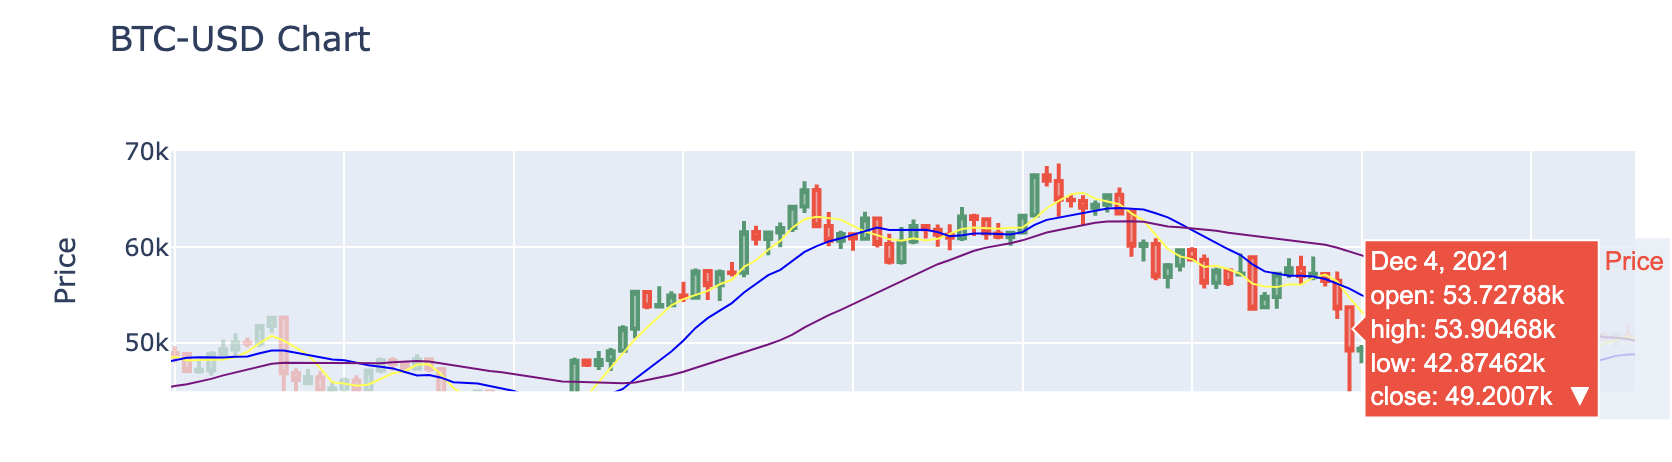
\includegraphics[width=1\linewidth]{Candlestick.png}
  \caption{Candlestick Chart.}
  \label{fig:example}
\end{figure}


6. Commodity Channel Index (CCI) Chart: This visualization will display the CCI of Bitcoin and Ethereum using a line chart. Users will be able to select the CCI period and view the CCI line along with the historical price movements of the crypto currencies.
\begin{figure}[!h]
  \centering
  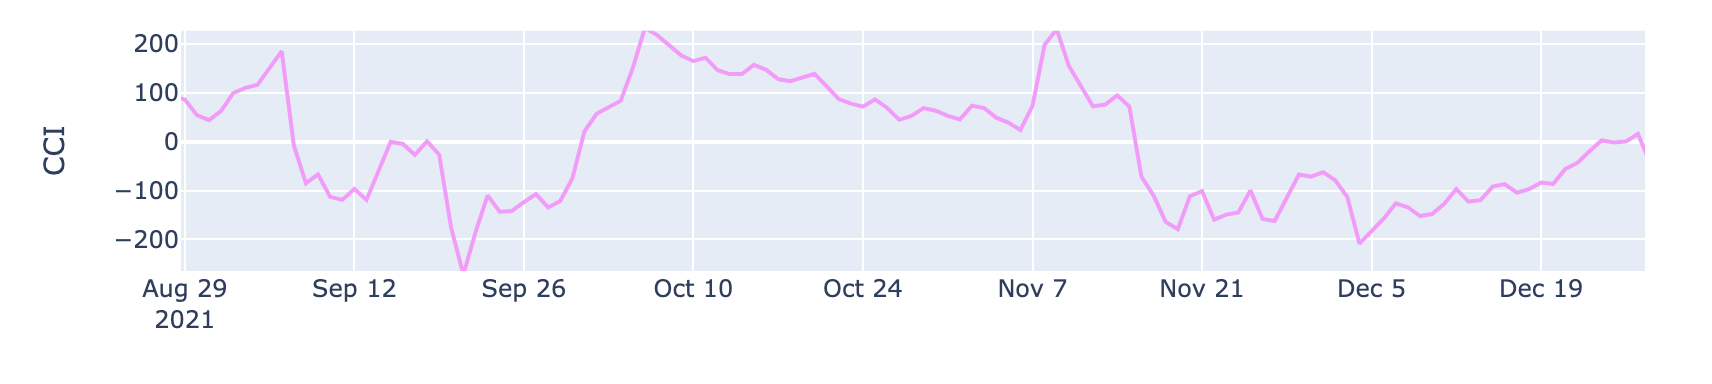
\includegraphics[width=1\linewidth]{CCI.png}
  \caption{Commodity Channel Index.}
  \label{fig:example}
\end{figure}


In addition to these visualizations, users will be able to customize the visualizations according to their preferences. They will be able to zoom in and out on the charts using the mouse scroll wheel, and they will be able to pan across the charts to view specific time frames. They will also be able to download the visualizations as image files for future reference or sharing.

Overall, the project's user interface will provide users with an easy-to-use and informative tool for analyzing the historical trends of Bitcoin and Ethereum, as well as several additional parameters such as MACD, MA, trading candlestick, and CCI. The visualizations will enable users to gain a better understanding of the performance of these crypto currencies over time, and make more informed decisions.

\section{Implementation}

3.1 Collection and Preprocessing of Data
For the purpose of analyzing Bitcoin and Ethereum's historical trends, the initiative will collect information from reputable sources such as crypto currencies exchanges and financial databases\cite{adithyan_2021}. For both crypto currencies, the data will include transaction prices, volumes, and dates. To ensure the accuracy of the visualizations, the collected data will be preprocessed to eradicate inconsistencies, missing values, and outliers.

3.2 Line Graph Displaying Historical Prices
The design of a line chart depicting the historical price movements of Bitcoin and Ethereum. The x-axis will represent time, while the y-axis will represent crypto currencies prices. The chart will exhibit two lines, one for each crypto currencies, each with a distinct color and label.

3.3 Stacked Area Chart of Volume Traded
The development of a piled area chart depicting the trading volume of Bitcoin and Ethereum over time. Time will be represented by the x-axis, while trading volume will be represented by the y-axis. The chart will depict two discrete areas, one for each crypto currencies, each with its own color and label.

3.4 The moving average (MA) chart and the moving average convergence divergence (MACD) chart will also be implemented using the same charting library. The MA and MACD values will be calculated based on the historical price data and formatted for use with the charting library. Controls will be added for selecting the MA period and the MACD parameters.

3.5 The candlestick chart will be implemented using a specialized charting library such as Highcharts or TradingView. The trading activity data will be fetched from the same reliable data source as before and formatted for use with the charting library. Interactivity will be added to the chart by allowing users to hover over the candlesticks to view specific price points and identify patterns and trends in the trading activity.

3.6 The commodity channel index (CCI) chart will also be implemented using the same charting library. The CCI values will be calculated based on the historical price data and formatted for use with the charting library. Controls will be added for selecting the CCI period.

3.7 User Interface Design
A user-friendly interface will be created using Python's Flask or Dash web framework to display the visualizations. The interface will include a menu for users to select different timeframes datasets and options to customize the visualizations according to their preferences. The line chart and stacked area chart will be placed side-by-side or vertically stacked to facilitate easy comparison between the two cryptocurrencies. Additionally, a brief description of each visualization and its significance will be provided to help users interpret the data.

3.8 Implementation
Python and various libraries will be used for data acquisition, analysis, and visualization on this project. To ensure interactive and responsive data visualizations, popular libraries such as Matplotlib and Plotly will be used to generate the visualizations.


%%%%%%%%%%%%%%%%%%%%%%%%%%%%%%%%%%%%%%%%%%%%%%%%%%%%%%%%%%%%%%%%%%%%
\section{Conclusion}

The aforementioned procedures were followed in order to construct an effective user interface for analysing the historical trends of Bitcoin and Ethereum, as well as various additional factors such as MACD, MA, trade candlesticks, and CCI. This allowed us to achieve our objective of implementing the user interface successfully. Users are provided with a simple-to-use, user-friendly instrument for gaining valuable insights into the performance of various crypto currencies over time. The user interface is designed to be informative and user-friendly. We anticipate that anyone interested in the cryptocurrency market will find this instrument informative and useful.
%%%%%%%%%%%%%%%%%%%%%%%%%%%%%%%%%%%%%%%%%%%%%%%%%%%%%%%%%%%%%%%%%%%%

{\small
\bibliographystyle{ieee}
\bibliography{references}
}
\end{document}
